\section{Mô hình VGG-16}
\subsection{Mô hình VGG16 là gì}
VGG là viết tắt của Visual Geometry Group; nó là một kiến trúc CNN sâu tiêu chuẩn với nhiều lớp. Kiến trúc VGG là cơ sở của các mô hình nhận dạng đối tượng mang tính đột phá. Được phát triển như một mạng nơ-ron sâu, VGGNet cũng vượt qua các đường cơ sở về nhiều tác vụ và bộ dữ liệu ngoài ImageNet. Hơn nữa, bây giờ nó vẫn là một trong những kiến trúc nhận dạng hình ảnh phổ biến nhất.

Karen Simonyan và Andrew Zisserman \cite{vgg16} đã đề xuất ý tưởng về mạng VGG vào năm 2013 và gửi mô hình thực tế dựa trên ý tưởng này trong ImageNet Challenge 2014. Họ gọi nó là VGG theo tên bộ phận của Visual Geometry Group tại Đại học Oxford nơi họ làm việc.

Mô hình VGG16, hoặc VGGNet, là một mạng nơ-ron phức hợp hỗ trợ 16 lớp. Mô hình VGG16 đạt được độ chính xác gần như 92,7\% trong bài kiểm tra top 5 trong ImageNet (ImageNet là một tập dữ liệu bao gồm hơn 14 triệu hình ảnh thuộc gần 1000 lớp), nó có thể phân loại hình ảnh thành 1000 loại đối tượng, bao gồm bàn phím, động vật, bút chì, chuột, v.v. Ngoài ra, mô hình có kích thước đầu vào hình ảnh là 224 x 224. Nó thay thế các bộ lọc kích thước hạt nhân lớn bằng một số bộ lọc kích thước hạt nhân 3 × 3 lần lượt.

\subsection{Cấu hình mô hình VGG16}
Trong tất cả các cấu hình, VGG16 được xác định là mô hình hoạt động tốt nhất trên tập dữ liệu ImageNet. Hãy xem lại kiến trúc thực tế của cấu hình này (Hình \ref{fig:vgg16_imagenet}).
\begin{figure}[H]
	\centering
	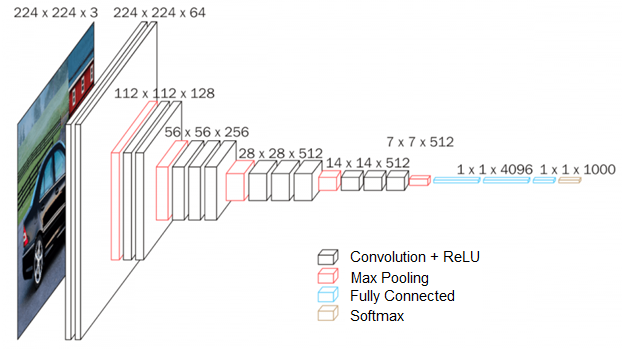
\includegraphics[width=0.6\linewidth]{images/vgg16_imagenet}
	\caption{Kiến trúc VGG16.}
	\label{fig:vgg16_imagenet}
\end{figure}
Đầu vào cho bất kỳ cấu hình mạng nào được coi là hình ảnh có kích thước cố định 224 x 224 với ba kênh R, G và B. Quá trình xử lý trước duy nhất được thực hiện là chuẩn hóa các giá trị RGB cho mỗi pixel. Điều này đạt được bằng cách trừ đi giá trị trung bình cho mỗi pixel.

Hình ảnh được chuyển qua ngăn xếp đầu tiên gồm 2 lớp tích chập có kích thước tiếp nhận rất nhỏ là 3 x 3, tiếp theo là kích hoạt ReLU. Mỗi lớp trong số hai lớp này chứa 64 bộ lọc. Stride được cố định ở 1 pixel và padding là 1 pixel. Cấu hình này bảo toàn độ phân giải không gian và kích thước của bản đồ kích hoạt đầu ra giống với kích thước hình ảnh đầu vào. Các bản đồ kích hoạt sau đó được chuyển qua tổng hợp tối đa không gian trên cửa sổ 2 x 2 pixel, với stride là 2 pixel. Điều này làm giảm một nửa kích thước của các lần kích hoạt. Do đó, kích thước của các kích hoạt ở cuối ngăn xếp đầu tiên là 112 x 112 x 64.

Các kích hoạt sau đó chảy qua ngăn xếp thứ hai tương tự, nhưng với 128 bộ lọc so với 64 bộ lọc trong ngăn xếp thứ nhất. Do đó, kích thước sau ngăn xếp thứ hai trở thành 56 x 56 x 128. Tiếp theo là ngăn xếp thứ ba với ba lớp chập và một lớp tổng hợp tối đa. Số lượng bộ lọc được áp dụng ở đây là 256, làm cho kích thước đầu ra của ngăn xếp là 28 x 28 x 256. Tiếp theo là hai ngăn xếp gồm ba lớp chập, với mỗi ngăn chứa 512 bộ lọc. Đầu ra ở cuối cả hai ngăn xếp này sẽ là 7 x 7 x 512.

Các chồng lớp chập trùng được theo sau bởi ba lớp được kết nối hoàn chỉnh với một lớp làm phẳng ở giữa. Hai lớp đầu tiên có 4.096 tế bào thần kinh mỗi lớp và lớp được kết nối đầy đủ cuối cùng đóng vai trò là lớp đầu ra và có 1.000 tế bào thần kinh tương ứng với 1.000 lớp có thể có cho tập dữ liệu ImageNet. Tiếp theo là lớp đầu ra là lớp kích hoạt Softmax được sử dụng để phân loại (Hình \ref{fig:vgg16_imagenet_detail}).

\begin{figure}[H]
	\centering
	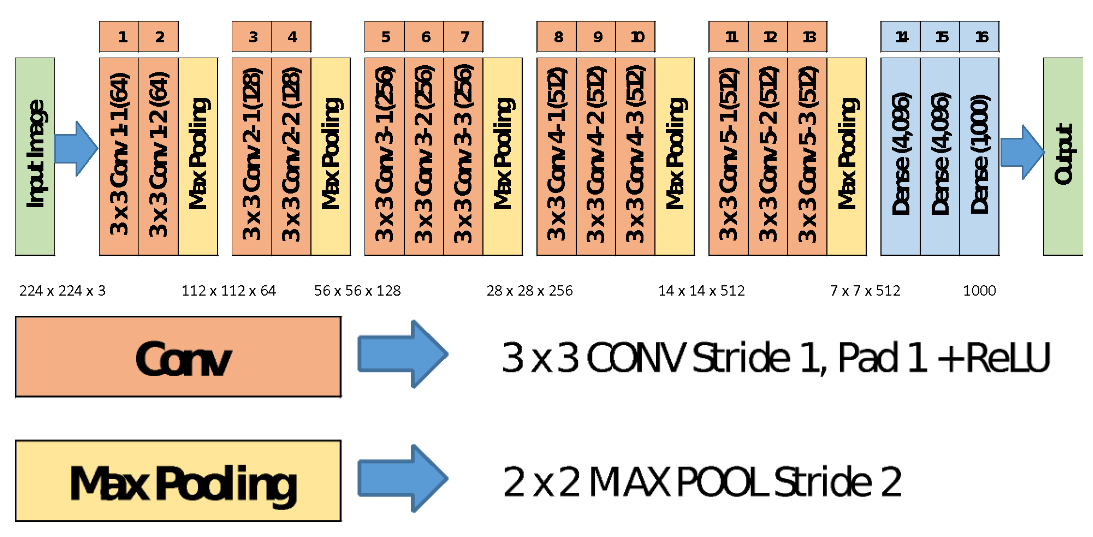
\includegraphics[width=1\linewidth]{images/vgg16_imagenet_detail}
	\caption{Chi tiết kiến trúc VGG16.}
	\label{fig:vgg16_imagenet_detail}
\end{figure}

\subsection{Cài đặt mô hình VGG16}
\begin{lstlisting}[language=Python]
	def make_vgg16_model(input_shape):
	inputs = keras.Input(shape=input_shape)
	x = data_augmentation(inputs)
	x = Rescaling(1.0 / 255)(x)
	#Block 1
	x = Conv2D(filters=start_step, kernel_size=(3, 3), padding='same', activation='relu', name='conv1_1')(x)
	x = Conv2D(filters=start_step, kernel_size=(3, 3), padding='same', activation='relu', name='conv1_2')(x)
	x = MaxPooling2D(pool_size=(2,2), strides=(2,2), name='max_pooling2d_1')(x)
	
	#Block 2
	x = Conv2D(filters=(start_step*2), kernel_size=(3, 3), padding='same', activation='relu', name='conv2_1')(x)
	x = Conv2D(filters=(start_step*2), kernel_size=(3, 3), padding='same', activation='relu', name='conv2_2')(x)
	x = MaxPooling2D(pool_size=(2,2), strides=(2,2), name='max_pooling2d_2')(x)
	
	#Block 3
	x = Conv2D(filters=(start_step*4), kernel_size=(3, 3), padding='same', activation='relu', name='conv3_1')(x)
	x = Conv2D(filters=(start_step*4), kernel_size=(3, 3), padding='same', activation='relu', name='conv3_2')(x)
	x = Conv2D(filters=(start_step*4), kernel_size=(3, 3), padding='same', activation='relu', name='conv3_3')(x)
	x = MaxPooling2D(pool_size=(2,2), strides=(2,2), name='max_pooling2d_3')(x)
	
	#Block 4
	x = Conv2D(filters=(start_step*8), kernel_size=(3, 3), padding='same', activation='relu', name='conv4_1')(x)
	x = Conv2D(filters=(start_step*8), kernel_size=(3, 3), padding='same', activation='relu', name='conv4_2')(x)
	x = Conv2D(filters=(start_step*8), kernel_size=(3, 3), padding='same', activation='relu', name='conv4_3')(x)
	x = MaxPooling2D(pool_size=(2,2), strides=(2,2), name='max_pooling2d_4')(x)
	
	#Block 5
	x = Conv2D(filters=(start_step*8), kernel_size=(3, 3), padding='same', activation='relu', name='conv5_1')(x)
	x = Conv2D(filters=(start_step*8), kernel_size=(3, 3), padding='same', activation='relu', name='conv5_2')(x)
	x = Conv2D(filters=(start_step*8), kernel_size=(3, 3), padding='same', activation='relu', name='conv5_3')(x)
	x = MaxPooling2D(pool_size=(2,2), strides=(2,2), name='max_pooling2d_5')(x)
	
	#Flatten and FC
	x = Flatten(name='flatten')(x)
	x = Dense((start_step*8), activation='relu', name='fc_1')(x)
	x = Dropout(0.5, name='dropout_1')(x)
	x = Dense((start_step*4), activation='relu', name='fc_2')(x)
	x = Dropout(0.5, name='dropout_2')(x)
	outputs = Dense(1, activation='sigmoid', name='output')(x)
	return keras.Model(inputs,outputs)			
\end{lstlisting}

\subsection{Ưu nhược điểm của mô hình VGG16}
\textbf{Ưu điểm:}
\begin{itemize}
	\item VGG đã mang đến một sự cải tiến lớn về độ chính xác và cải thiện cả về tốc độ. Điều này chủ yếu là do cải thiện độ sâu của mô hình.
	\item Sự gia tăng số lượng các lớp với các hạt nhân nhỏ hơn làm tăng tính phi tuyến tính, điều này luôn luôn là một điều tích cực trong học sâu.
	\item VGG mang theo nhiều kiến trúc khác nhau được xây dựng dựa trên khái niệm tương tự. Điều này cung cấp cho chúng ta nhiều lựa chọn hơn về kiến trúc nào có thể phù hợp nhất với ứng dụng của chúng ta.
\end{itemize}
\textbf{Nhược điểm:}
\begin{itemize}
	\item Một vấn đề của VGG liên quan đến giới hạn tính toán của máy tính cũng khiến cho việc huấn luyện không hiệu quả khi số lượng hidden layers lớn lên. Vấn đề này có tên là vanishing gradient.
	\item Số lượng bộ lọc mà chúng ta có thể sử dụng tăng gấp đôi trên mỗi bước hoặc qua mỗi ngăn xếp của lớp tích chập. Đây là một nguyên tắc chính được sử dụng để thiết kế kiến trúc của mạng VGG16. Một trong những nhược điểm quan trọng của mạng VGG16 là nó là một mạng khổng lồ, có nghĩa là cần nhiều thời gian hơn để đào tạo các tham số của nó.
\end{itemize}
